\documentclass[border=10pt]{standalone}
\usepackage{tikz}
\usetikzlibrary{shapes, arrows.meta, positioning, fit, backgrounds, shadows}

\definecolor{softblue}{RGB}{232, 241, 250}
\definecolor{softgreen}{RGB}{230, 244, 234}
\definecolor{softred}{RGB}{252, 232, 230}
\definecolor{softyellow}{RGB}{254, 247, 224}
\definecolor{bordergray}{RGB}{100, 100, 100}

\begin{document}
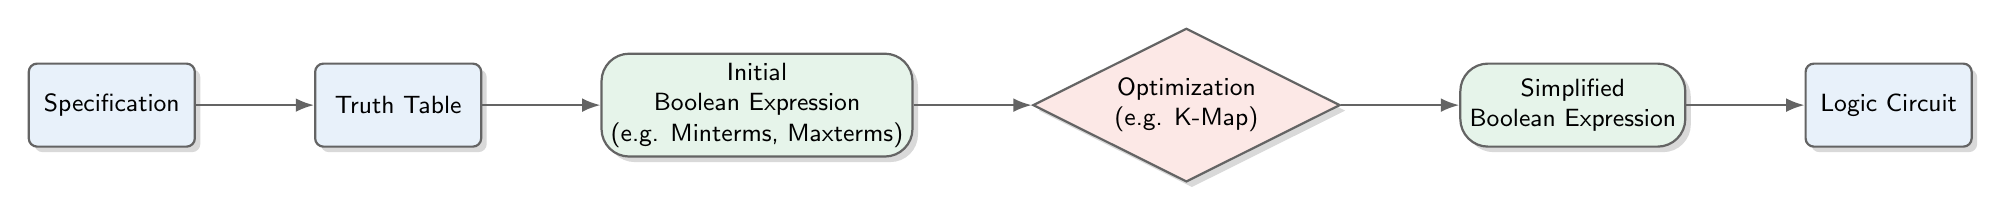
\begin{tikzpicture}[
    node distance=1.0cm and 1.5cm,
    font=\sffamily\small,
    base/.style={
        draw=bordergray, 
        thick, 
        align=center, 
        drop shadow={opacity=0.3, shadow xshift=2pt, shadow yshift=-2pt}
    },
    block/.style={
        base, 
        rectangle, 
        rounded corners=3pt, 
        minimum height=3em, 
        minimum width=6em, 
        fill=softblue
    },
    rounded_block/.style={
        base, 
        rectangle, 
        rounded corners=1em, 
        minimum height=3em, 
        minimum width=6em, 
        fill=softgreen
    },
    decision/.style={
        base, 
        diamond, 
        aspect=2, 
        minimum height=3em, 
        minimum width=6em, 
        fill=softred
    },
    arrow/.style={-Latex, thick, color=bordergray}
]

    % Nodes
    \node[block] (spec) {Specification};
    \node[block, right=of spec] (truth_table) {Truth Table};
    \node[rounded_block, right=of truth_table] (init_expr) {Initial\\Boolean Expression\\(e.g. Minterms, Maxterms)};
    \node[decision, right=of init_expr] (opt) {Optimization\\(e.g. K-Map)};
    \node[rounded_block, right=of opt] (simp_expr) {Simplified\\Boolean Expression};
    \node[block, right=of simp_expr] (circuit) {Logic Circuit};

    % Edges
    \draw[arrow] (spec) -- (truth_table);
    \draw[arrow] (truth_table) -- (init_expr);
    \draw[arrow] (init_expr) -- (opt);
    \draw[arrow] (opt) -- (simp_expr);
    \draw[arrow] (simp_expr) -- (circuit);

\end{tikzpicture}
\end{document}
